
In this section we show that the \carpool problem can be formulated as
unconstrained submodular maximization problem, and thus it has a
randomized $\frac{1}{2}$-approximation algorithm based on~\cite{BFNS15}.

Given a \carpool instance $(G = (V,A), c, w)$, consider a subset
$S \subseteq V$.  Let $M(S)$ be the maximum weight carpool matching
that satisfies $D_{M(S)} \subseteq S \subseteq V \setminus P_{M(S)}$,
namely $M(S)$ is the best carpool matching whose drivers belong to $S$
and whose passengers belong to $V \setminus S$.  In other words,
$M(S)$ is the maximum weight carpool matching that is a subset of
$A \cap (V \setminus S) \times S$.
%
Given $S$, the carpool matching $M(S)$ can be computed in polynomial
time using a maximum b-matching in the bipartite graph 
$B = (S \cup V \setminus S, A \cap (V \setminus S) \times S)$ or can be reduced
to a max-cost flow problem as shown in~\cite{kutiel2016}.

Consider the function $\barw: 2^V \to \R$, where $\barw(S) \eqdf
w(M(S))$.  In the next lemma we prove that $\bar{w}$ is
a \emph{submodular set function}.  Recall that a function $f$ is
submodular if $f(S) + f(T) \geq f(S \cup T) + f(S \cap T)$ for every
two sets $S$ and $T$ in the domain of $f$.

\begin{lemma}
$\barw$ is submodular.
\end{lemma}
\begin{proof}
Consider any two subsets $S, T \subseteq V$.  We show that $\barw(S)
+ \barw(T) \geq \barw(S \cup T) + \barw(S \cap T)$.
%
Let $M(S \cup T)$ and $M(S \cap T)$ be the optimal carpool matchings
with respect to $S \cup T$ and $S \cap T$, respectively.
%
To prove the lemma we construct two feasible carpool matchings $M_S$
and $M_T$ such that $M_S \subseteq (V \setminus S) \times S$,
$M_T \subseteq (V \setminus T) \times T$, and $M_S \cup M_T = M(S \cup
T) \cup M(S \cap T)$.

First, add all the edges in $M(S \cup T)$ entering $S \setminus T$ to
$M_S$.  Similarly, add all the edges in $M(S \cup T)$ entering
$T \setminus S$ to $M_T$.  Observe that $\din[M_S](v) = \din[M(S \cup
T)](v) \leq c(v)$, for every $v \in S \setminus T$ and that
$\din[M_T](v) = \din[M(S \cup T)](v) \leq c(v)$, for every $v \in
T \setminus S$.

Next, add the edges in $M(S \cap T)$ leaving $T \setminus S$ to $S$
and add the edges in $M(S \cap T)$ leaving $S \setminus T$ to $T$.
%
It remains to distribute the edges leaving $V \setminus (S \cup T)$
and entering $S \cap T$ in both $M(S \cup T)$ and $M(S \cap T)$.  Note
that there may exist edges $(v,u)$, where $v \not\in S \cup T$, and
$u \in S \cap T$ such that $(v,u) \in M(S \cup T)$ and $M(S \cap T)$.
We refer to this edges as \emph{duplicate} edges.
%
We add all edges leaving $V \setminus (S \cup T)$ and entering $S \cap
T$ in $M(S \cap T)$ to $M_S$.  Notice that this is possible, since
after this addition we have that $\din[M_S](v) \leq \din[M(S \cap
T)](v) \leq c(v)$, for every vertex $v \in S \cap T$.
%
Then we add all duplicate edges in $M(S \cup T)$ to $M_T$.
%
The remaining edges are distributed between $M_S$ and $M_T$ without
violating capacities.  This can be done, since $\din[M(S \cup T)](v)
+ \din[M(S \cap T)](v) \leq 2c(v)$, for every $v \in S \cap T$.

The lemma follows, since $\barw(S) \geq w(M_S)$ and $\barw(T) \geq
w(M_T)$.
\end{proof}

Buchbinder et al.~\cite{BFNS15,buchbinder2016deterministic} presented a
general randomized $2$-approximation algorithm for unconstrained submodular maximization.

\begin{theorem}
There exists a polynomial time $2$-approximation algorithm for \carpool.
\end{theorem}

\begin{figure}
\centering
\begin{subfigure}{.45\linewidth}
\centering
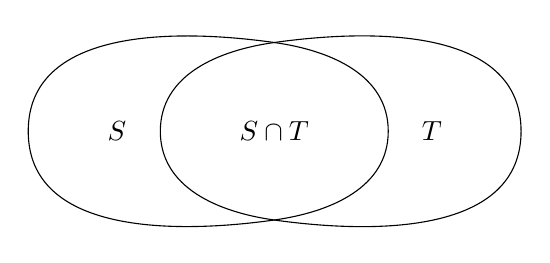
\begin{tikzpicture}[]

\begin{scope}[every node/.style={inner sep=1cm}]
\node(s) at(-2,0) {$S$};
\node(st) at(0,0) {$S \cap T$};
\node(t) at(2,0) {$T$};
\end{scope}

\draw 
(s.west) to[out=90, in=172] 
(st.north) to[out=-8, in=90] 
(st.east) to[out=270, in=8]
(st.south) to[out=188, in=270]
(s.west)
;

\draw 
(t.east) to[out=90, in=8] 
(st.north) to[out=188, in=90] 
(st.west) to[out=270, in=172]
(st.south) to[out=-8, in=270]
(t.east)
;

\end{tikzpicture}
\end{subfigure}
%
\hfill
%
\begin{subfigure}{.45\linewidth}
\centering
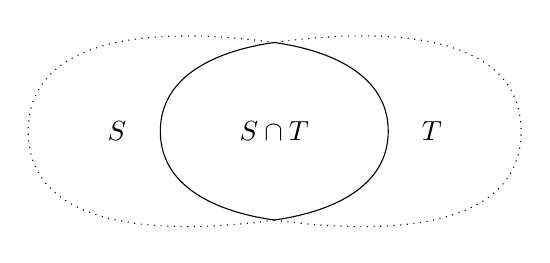
\begin{tikzpicture}[]

\begin{scope}[every node/.style={inner sep=1cm}]
\node(s) at(-2,0) {$S$};
\node(st) at(0,0) {$S \cap T$};
\node(t) at(2,0) {$T$};
\end{scope}

\draw[dotted] 
(st.south) to[out=188, in=270]
(s.west) to[out=90, in=172] 
(st.north)
;
\draw 
(st.north) to[out=-8, in=90] 
(st.east) to[out=270, in=8]
(st.south)
;

\draw[dotted] 
(st.south) to[out=-8, in=270]
(t.east) to[out=90, in=8] 
(st.north)
;
\draw 
(st.north) to[out=188, in=90] 
(st.west) to[out=270, in=172]
(st.south)
;

\end{tikzpicture}
\end{subfigure}

\begin{subfigure}{.45\linewidth}
\centering
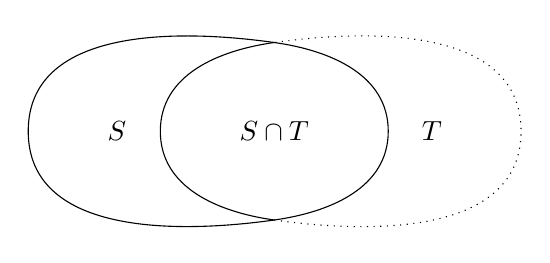
\begin{tikzpicture}[]

\begin{scope}[every node/.style={inner sep=1cm}]
\node(s) at(-2,0) {$S$};
\node(st) at(0,0) {$S \cap T$};
\node(t) at(2,0) {$T$};
\end{scope}

\draw 
(s.west) to[out=90, in=172] 
(st.north) to[out=-8, in=90] 
(st.east) to[out=270, in=8]
(st.south) to[out=188, in=270]
(s.west)
;

\draw[dotted] 
(st.south) to[out=-8, in=270]
(t.east) to[out=90, in=8] 
(st.north) 
;
\draw 
(st.north) to[out=188, in=90] 
(st.west) to[out=270, in=172]
(st.south)
;

\end{tikzpicture}
\end{subfigure}
%
\hfill
%
\begin{subfigure}{.45\linewidth}
\centering
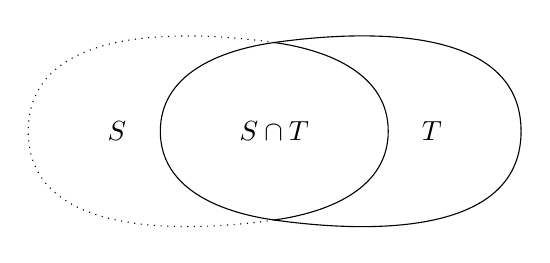
\begin{tikzpicture}[]

\begin{scope}[every node/.style={inner sep=1cm}]
\node(s) at(-2,0) {$S$};
\node(st) at(0,0) {$S \cap T$};
\node(t) at(2,0) {$T$};
\end{scope}

\draw[dotted] 
(st.south) to[out=188, in=270]
(s.west) to[out=90, in=172] 
(st.north)
;
\draw 
(st.north) to[out=-8, in=90] 
(st.east) to[out=270, in=8]
(st.south)
;

\draw 
(t.east) to[out=90, in=8] 
(st.north) to[out=188, in=90] 
(st.west) to[out=270, in=172]
(st.south) to[out=-8, in=270]
(t.east)
;

\end{tikzpicture}
\end{subfigure}
\caption[]{
\label{fig:defs}
We show that the arcs from \subref{sub:cup} and \subref{sub:cap} can be
redistributed over \subref{sub:s} and \subref{sub:s} 
%\todo{write explanation}
}
\end{figure}
